\scanpage{165}
\margin{$\operatorname{cdim\,inj}F\leq 2\dim\unsure{\operatorname{Supp}F|X_{\operatorname{Supp}F}}+\sup_{x\in X}\dim\operatorname{inj}F_{\bar{x}}$}
\begin{center}
INSTITUT\\
DES HAUTES ÉTUDES SCIENTIFIQUES
\end{center}
\uline{Applications} --- \uline{possibles}

\textcircled{1} Majoration de la cdim. inj. via la dim inj. des fibres

Dim. ch. \unsure{stricte|stricts} d'un préschéma (en particulier d'un pr. Alg.)

(Consulter notes de Verdier)
\margin{$\operatorname{c-dim\,inj}(F)\leq\displaystyle\sup_{x\in X,\,F_{\bar{x}}\ne0}\left[2\dim O_{X,\bar{x}}+\dim\operatorname{inj}F_{\bar{x}}\right]$}

\figure{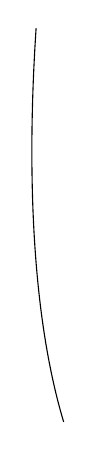
\begin{tikzpicture}[x=1cm,y=1cm]
\draw (0,0)..controls(-.1,-1.5) and (-.1,-3.5)..(.35,-5.0);
\end{tikzpicture}}
\textcircled{2} Cas d'un Anneau $A$ de torsion \uline{loc.} \uline{ct} premier aux car. résiduelles, et $R_X$ complexe de faisceaux de $A_X$-modules \unsure{\{}loc. cts, dualisant fibre par fibre (sur $X$ régulier ---)

\uline{NB} On peut globaliser, et considérer des schémas relatifs sur $(X_{\text{ét}},(\mathbb{Z}/n\mathbb{Z})_X)$ ----.

\textcircled{3} \deleted{Applications aux ths. de Lefschetz cohomologiques locaux et globaux [\unsure{Pourrait|Pourrais} donner un article séparé ....]}
\margin{164}
